% Physicist-facing status report on gauge-covariant VFE renormalization.
% Standalone; companion to solid_RG_theory.tex and Theory/main.tex.
\documentclass[11pt,letterpaper]{article}

\usepackage[margin=1in]{geometry}
\usepackage{amsmath,amssymb,mathtools}
\usepackage{bm}
\usepackage{booktabs}
\usepackage{xcolor}
\usepackage{microtype}
\usepackage{tikz}
\usetikzlibrary{calc,arrows.meta,positioning,fit,backgrounds,shapes.geometric}
\usepackage[hidelinks]{hyperref}

\newcommand{\KL}{D_{\mathrm{KL}}}
\newcommand{\E}{\mathbb E}
\newcommand{\push}{_{\#}}
\newcommand{\Fen}{\mathcal F}

\definecolor{estab}{RGB}{38,92,150}
\definecolor{openc}{RGB}{176,64,52}
\definecolor{softg}{RGB}{237,240,244}
\definecolor{parent}{RGB}{58,124,88}

\title{The State of Gauge-Covariant VFE Renormalization\\
\large A status report for physicists}
\author{Gauge-Theoretic Multi-Agent Variational Free-Energy Program}
\date{August 2026}

\begin{document}
\maketitle

\begin{abstract}
This note summarizes what the gauge-covariant variational free-energy program has
actually established about renormalization, what it has not, and which obligations
block progress. The short version is that an exact finite coarse-graining calculus
has been derived under explicit hypotheses and internally checked, while a
renormalization \emph{group} has not yet been constructed: there is no endogenous
rescaling map, RG beta function, blocking ratio, or relevant--irrelevant
classification for the two-channel gauge network. Recent work has sharpened three
things worth knowing. With an unrestricted copy-capable parent and downward-kernel
family, descent of the multiscale free energy ranks no partition. After
Perron-occupancy symmetrization of an irreducible chain, the directed edge-event law
supplies an intrinsic gauge-invariant graph metric and diffusion scale where the
attention weights do not. And nontrivial holonomy on a cyclic graph can make a
zero-distortion parent nonexistent within a declared admitted family. Persistence,
emergent hierarchy, and physical RG flow remain unproved.
\end{abstract}

\section{Where things stand}

The program's object of study is a finite population of agents that each carry two
statistical presentations, a belief and a generative model, transported between
agents by two generally different gauge connections. The question is whether such a
population organizes itself into a hierarchy of meta-agents under descent of a
single variational free energy, and whether that hierarchy constitutes a
renormalization group.

The answer at present separates cleanly into three layers. The exact finite layer
has explicit derivations under stated hypotheses and has been internally checked,
but the current multiscale package remains formally \textsc{inconclusive} rather
than independently claim-verified. This layer includes normalized coarse-graining
channels, the free-energy identity they satisfy, the construction of a parent from
a block of children, the correct way to coarse-grain directed attention, and the
exact treatment of non-flat connection data. In the unrestricted copy-capable
family, the selection layer is degenerate: the free energy is exactly indifferent
to the choice of partition unless extra structure is declared. Block persistence,
closure across scales, and any identification of the descent parameter with physical
time remain open, and the project's own claim ledger has said so consistently.

What has changed recently is mostly negative in the productive sense. Several
plausible shortcuts have been closed off by explicit counterexamples rather than
left as caveats, and an external review found four substantive defects in the most
recent derivation package, all of which are now repaired. That is progress of the
kind worth having, but it is not progress toward a renormalization group.

\section{The object: one free energy, two channels}

Fix structural data $X$ containing the finite directed interaction skeleton, which
may contain cycles, and fix an observation record $o$. All scale-zero agents sit at
one contextual point, so there is no ambient length, no lattice, no translation
symmetry, and no momentum space to organize a Wilsonian scheme. Let $W$ collect
every random object the multiscale model retains: belief and model presentations at
every scale, the directed weights, the receiver occupancies, the two channels'
transports, the partition variables, and the retained holonomy marks.

Declare one normalized generative law $\mathbb P_\theta(do,dW\mid X)$, fixed before
inference runs, and one normalized correlated recognition law
$\mathbb Q_\phi(dW\mid o,X)$. The entire theory is the single identity
\begin{equation}
\Fen_{\mathrm{tower}}
= -\log p_\theta(o\mid X)
+ \KL\!\left(\mathbb Q_\phi \,\middle\Vert\, \bm\Pi_{\theta,o,X}\right),
\label{eq:vfe}
\end{equation}
where $\bm\Pi$ is the posterior. The evidence term plays the role of a fixed baseline for the
record: fixed once the model and the observation are fixed, and immovable by
variational work. The divergence is the only thing descent can lower.

Every familiar-looking piece of a multi-agent free energy, meaning a self term, an
edge term, a partition term, or a parent--child term, is legitimate only as an
accounting split of that one divergence, obtained by factorizing the two laws along
a common ordering. A sum of such pieces assembled by hand is a composite descent
potential. It may be a perfectly good objective, but it is not an evidence bound, it
does not inherit the floor $\Fen \ge -\log p$, and its stationary points carry no
Bayesian reading. This distinction does real work below.

Two structural facts about \eqref{eq:vfe} deserve emphasis. First, because every
factor in the generative law is a normalized transition kernel of finite scope, the
tower requires no additional global Gibbs partition function beyond the evidence;
the normalized kernels retain their own declared local normalization. Local
normalization of node and edge potentials does not by itself give a finite global
normalizer, as the Gaussian pair with edge potential $e^{c y_1 y_2}$ shows: its
precision loses positive definiteness at $c\ge1$, with a zero eigenvalue at $c=1$
and a negative eigenvalue for $c>1$. Any same-time reciprocal
coupling between scales reintroduces that obligation and must discharge it. Second,
no generative factor may read the recognition law or the posterior it is supposed to
determine. Violating this turns the model into a family indexed by the recognition
law, in which no member is distinguished and a divergence decrease certifies nothing
about evidence.

\subsection{The typing fork that decides whether attention is an ELBO term}

The transported disagreement between neighbors is written
\begin{equation}
D^b_{ij} = \KL\!\left(q^b_i \,\middle\Vert\, (\Omega^b_{ij})\push q^b_j\right),
\qquad
D^m_{ij} = \KL\!\left(q^m_i \,\middle\Vert\, (\Omega^m_{ij})\push q^m_j\right).
\end{equation}
Whether the associated row free energies are part of the evidence bound depends
entirely on what kind of object $q^b_i$ is, and this is the most common source of
confusion in the program.

If the agent's latent variable \emph{is} a law, so that $q^b_i$ is a point of the
statistical fiber and a component of the sample, then $D^b_{ij}$ is a function of
the state and may legitimately appear inside a generative likelihood factor. Under
that reading, plus a label-exclusivity hypothesis on an augmented source label and a
restriction of the recognition law to constant rows, define the familiar row
functional
\begin{equation}
\Phi^b_i = \sum_j \beta_{ij} \E_{\mathbb Q} D^b_{ij}
+ \tau^b_i \KL(\beta_i \Vert \pi^b_i)
\end{equation}
with softmax optimum
$\beta^\star_{ij} \propto \pi_{ij} \exp(-\E_{\mathbb Q} D_{ij}/\tau_i)$. Note the
expectation: the energy is the recognition average of the transported divergence,
not the divergence evaluated at an average, and the two differ unless the state law
is degenerate. The exact categorical VFE sector is $\tau_i^{-1}\Phi_i$. Thus
$\Phi_i$ has the same optimizer, but for $\tau_i\ne1$ it is not an independently
weighted sector of one standard ELBO unless the entire objective is scaled or a
different generalized free energy is declared.

If instead $q^b_i$ denotes the recognition marginal, then $D^b_{ij}$ is a functional
of the recognition law, inserting it into a generative factor violates the typing
prohibition, and everything assembled from it is a composite potential rather than a
bound. Both readings appear in the program's own documents, which is why stating
which one is in force matters more than it looks.

\section{The exact layer, which works}

\begin{figure}[t]
\centering
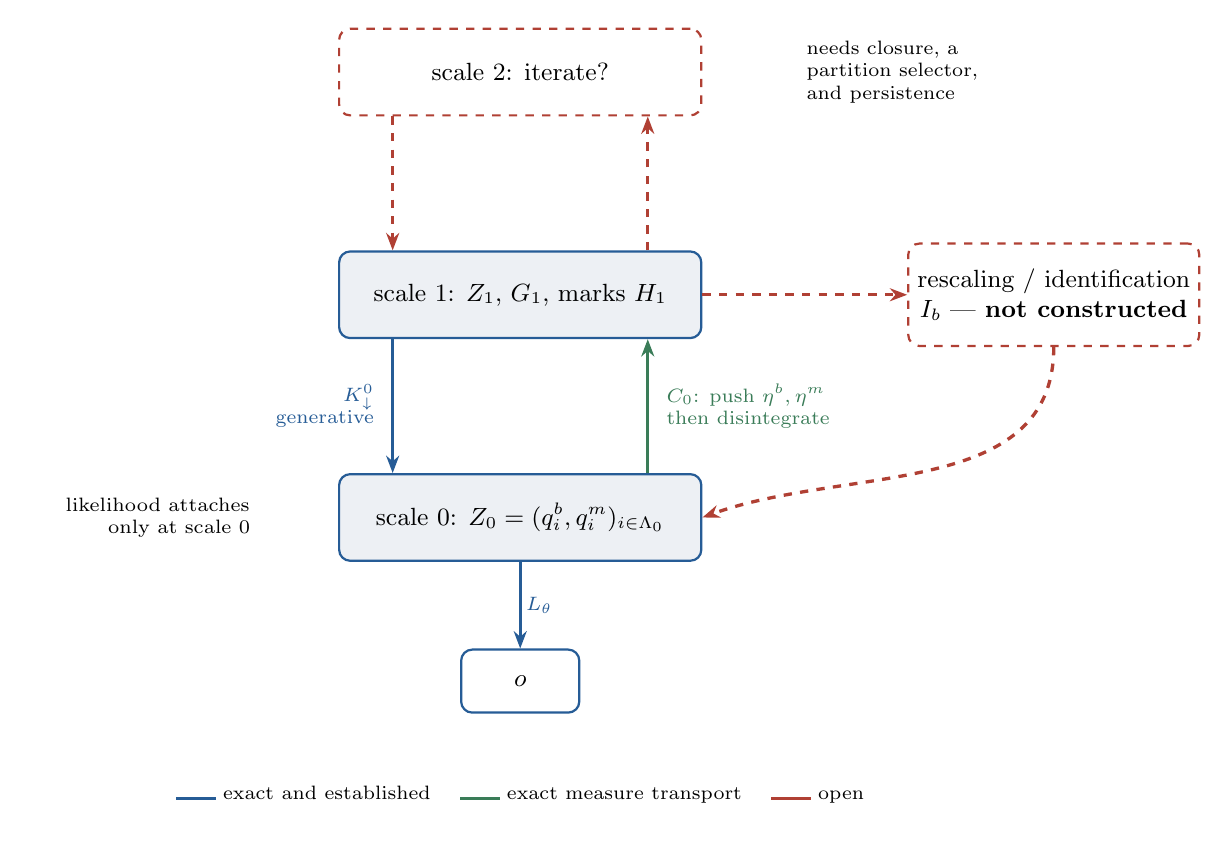
\begin{tikzpicture}[
  >={Stealth[length=2.2mm]},
  every node/.style={font=\small},
  lvl/.style={draw=estab, thick, rounded corners, fill=softg,
              minimum width=46mm, minimum height=11mm, align=center},
  lvlopen/.style={draw=openc, thick, dashed, rounded corners, fill=white,
                  minimum width=46mm, minimum height=11mm, align=center},
  down/.style={->, estab, very thick},
  up/.style={->, parent, very thick},
  gap/.style={->, openc, very thick, dashed},
]
\node[lvl] (s0) at (0,0) {scale $0$: $Z_0=(q^b_i,q^m_i)_{i\in\Lambda_0}$};
\node[lvl, above=17mm of s0] (s1) {scale $1$: $Z_1$, $G_1$, marks $H_1$};
\node[lvlopen, above=17mm of s1] (s2) {scale $2$: iterate?};

\node[draw=estab, thick, rounded corners, fill=white,
      minimum width=15mm, minimum height=8mm, below=11mm of s0] (obs) {$o$};
\draw[down] (s0) -- node[right, font=\scriptsize, inner sep=1.5pt] {$L_\theta$} (obs);

\draw[down] ($(s1.south west)!0.30!(s1.south)$) --
            node[left, font=\scriptsize, align=right, xshift=-1mm]
            {$K_\downarrow^{0}$\\generative}
            ($(s0.north west)!0.30!(s0.north)$);
\draw[gap]  ($(s2.south west)!0.30!(s2.south)$) --
            ($(s1.north west)!0.30!(s1.north)$);

\draw[up] ($(s0.north east)!0.30!(s0.north)$) --
          node[right, font=\scriptsize, align=left, xshift=1mm]
          {$C_0$: push $\eta^{b},\eta^{m}$\\then disintegrate}
          ($(s1.south east)!0.30!(s1.south)$);
\draw[gap] ($(s1.north east)!0.30!(s1.north)$) --
           ($(s2.south east)!0.30!(s2.south)$);

\node[draw=openc, thick, dashed, rounded corners, fill=white,
      align=center, minimum height=13mm, right=26mm of s1] (Ib)
      {rescaling / identification\\$I_b$ \textemdash{} \textbf{not constructed}};
\draw[gap] (s1.east) -- (Ib.west);
\draw[gap] (Ib.south) to[out=-90, in=20] (s0.east);

\node[below=8mm of obs, align=left, font=\scriptsize] (leg) {%
  \textcolor{estab}{\rule{5mm}{1.1pt}}~exact and established \quad
  \textcolor{parent}{\rule{5mm}{1.1pt}}~exact measure transport \quad
  \textcolor{openc}{\rule{5mm}{1.1pt}}~open};

\node[left=10mm of s0, align=right, font=\scriptsize, text width=27mm] {%
  likelihood attaches\\only at scale $0$};
\node[right=6mm of s2, align=left, font=\scriptsize, text width=30mm, xshift=6mm] {%
  needs closure, a\\partition selector,\\and persistence};
\end{tikzpicture}
\caption{\textbf{The scale ladder and the missing piece.} Generation runs downward
through normalized kernels $K_\downarrow$, with the likelihood attached only at the
finest scale. Coarse-graining runs upward and acts on \emph{measures}, pushing the
directed edge-event laws through one normalized channel and then disintegrating. Both
directions are exact. What has not been constructed is the rescaling and identification map
$I_b$ that would return the coarse description to a common comparison space, and
without it the family of coarse-grainings never becomes a semigroup.}
\label{fig:ladder}
\end{figure}

Figure~\ref{fig:ladder} shows the architecture. Several results in it are exact and
settled, and they are worth stating plainly because they are the parts a physicist
can build on.

\paragraph{Coarse-graining is a controlled loss.} Apply one normalized channel $C$,
which must not read the recognition law, to both the recognition law and the
posterior, leaving the observation untouched. Then
\begin{equation}
\Fen_P(Q_o) = \Fen_{P^c}(Q^c_o) + \Delta,
\qquad
\Delta = \int \KL\!\left(\widehat Q_o(dy \mid z) \,\middle\Vert\,
\widehat\Pi_o(dy \mid z)\right) Q^c_o(dz) \ \ge 0,
\end{equation}
as an additive identity valid even when terms are infinite. The coarse free energy
is lower, and the discarded quantity $\Delta$ is exactly the conditional information
thrown away. It vanishes precisely when the discarded conditional recognition and
posterior laws agree. This is the correct statement of ``coarse-graining lowers the
free energy'' in this theory, and it must not be read as model improvement.

\paragraph{A block of children defines a parent.} Given a block and one normalized
channel independent of recognition, the generative law, the posterior, and the
recognition law all push forward to a normalized parent triple with the same
evidence. The parent's belief and model laws are coordinate projections of that
triple. They do not reconstruct it: two different joint laws can share all their
coordinate marginals, so a meta-agent defined only by its transported belief
marginal is underdetermined.

\paragraph{Directed attention coarse-grains through the event law, not the rows.}
A row $\beta_{ij}$ is a conditional law of a source given a receiver and cannot be
coarse-grained alone. The transportable object is the joint directed edge-event law
$\eta^b_{ij} = \alpha^b_i \beta_{ij}$ and its model-channel partner, which are
gauge-invariant scalars. Coarse rows are obtained by pushing the event law through a
normalized endpoint kernel and then disintegrating,
\begin{equation}
\eta^{c}_{AB} = \sum_{i,j} \eta_{ij} K(A,B \mid i,j),
\qquad
\alpha^c_A = \sum_B \eta^c_{AB},
\qquad
\beta^c_{AB} = \eta^c_{AB} / \alpha^c_A ,
\end{equation}
on positive parent occupancy. Averaging the rows instead is simply wrong, and the
error is not small: a three-node example with skewed occupancy gives $0.9$ against
$0.5$ for the same coarse entry.

\paragraph{Exact closure generates many-body terms.} Eliminating internal variables
exactly produces the full hyperedge family, recoverable by inclusion--exclusion.
Pairwise closure is false in general, as the Ising star shows by producing a nonzero
three-body coefficient $2\,\mathrm{sech}^2(h_0)\tanh(h_0) J_1 J_2 J_3$ at leading
order whenever the field and all three couplings are nonzero. Any pairwise coarse
theory is therefore a truncation carrying a residual, not an exact effective theory.

\paragraph{Non-flat connections are retained, not averaged away.} The exact coarse
connection datum is the conditional \emph{law} of the dressed microscopic transports
$\Theta^{IJ}_{ij} = \Omega_{Ii}\Omega_{ij}\Omega_{jJ}$, together with the based
holonomy representation and the dressed boundary generators in one simultaneous
root-gauge orbit. A mean will not substitute for it. The average of a rotation by
$+\pi/2$ and one by $-\pi/2$ is the zero matrix, which is not a group element at all,
so ``the coarse edge transport'' generically does not exist as a single group
element. Correlations make matters worse: marks and features with vanishing separate
means can have a nonvanishing mean product.

\section{Why there is no renormalization group}

A renormalization step is a coarse-graining \emph{plus} a rescaling that returns the
coarse description to a common space where it can be compared with the original.
Only then does one get a semigroup $K_{b_1 b_2} = K_{b_1} K_{b_2}$, a flow on a space
of couplings, fixed points, and a classification of directions as relevant or
irrelevant.

The program has the first half and not the second. Coarse channels compose,
$C_{20} = C_{21} C_{10}$, so there is a consistent family of coarse-grainings indexed
by nested partitions. There is no rescaling or identification map. The closure
theorem in the manuscript does derive discrete beta functionals, but it assumes such
rescaling kernels among its hypotheses rather than constructing them, and it carries
the reminder that a beta functional is a joint statement about the action \emph{and}
a declared reference trajectory: changing the reference shifts beta by an
inhomogeneous term that is not a reparameterization. There is likewise no blocking
ratio, since blocks are labeled by partitions rather than by a scale factor, and no
relevant--irrelevant classification, since that requires a linearization about a
fixed point that has not been exhibited. The only fixed point named anywhere in the
finite theory is the contextual base point, which is a chosen location and not a
fixed point of any flow.

This is worth stating bluntly because the vocabulary of renormalization is used
throughout the program's documents, and the vocabulary is currently aspirational.

\section{Four recent sharpenings}

\subsection{The free energy ranks no partition}

The most consequential recent result is negative. Suppose the parent space and the
downward kernel family are unrestricted, in the sense that one may take the parent
space to be a copy of the child space and the downward kernel to be the identity. Then
for \emph{every} partition, including all-singletons and one-big-block, the minimized
tower free energy equals $-\log p^{\mathrm{flat}}(o \mid X)$, the same number. The
minimum depends on the partition only through the observation marginal, and the copy
construction leaves that marginal untouched.

The consequence is sharp. The inferred distribution over partitions equals its prior,
the data contribute nothing, and any claim that a hierarchy ``emerges from the
variational principle'' is vacuous in that regime. Selection must come from declared
structure: a capacity restriction on the parent space and kernel family, which
penalizes one big block by making it unable to represent its children, together with
a cost per parent node, which penalizes all-singletons. Both are sufficient
mechanisms aimed at the two degeneracies. Whether both are \emph{necessary} over some
declared class of models is open, and the earlier claim that they were has been
withdrawn.

\subsection{A genuine gauge-invariant length scale}

The heuristic reading of $1/\beta_{ij}$ as an interaction length does not survive
scrutiny. It is directed, it is competitive because raising one entry lowers the
others through row normalization, it diverges as the weight vanishes, and it obeys no
triangle inequality. The Gibbs-optimal surprisal inherits all of these.

There is a good replacement built from the same data. Since the edge-event law and
the occupancies are gauge-invariant scalars,
\begin{equation}
L^x = \operatorname{diag}(\alpha^x) - \eta^x
\end{equation}
is gauge-invariant and has exactly zero row sums, so it generates an honest diffusion
rather than a killed one. If the receiver occupancy is chosen self-consistently as the
stationary vector of the attention chain, then the additive symmetrization of the
edge-event law preserves the occupancy exactly and coincides with the standard
symmetrization used to define a directed graph Laplacian. On each connected component
of the resulting symmetric operator, effective resistance and commute time \emph{are}
metrics; across components they are naturally treated as infinite extended distances.
A diffusion time at which the entropic susceptibility peaks supplies an intrinsic
candidate scale that requires no ambient embedding. Running the two channels
separately gives two scale spectra, and their disagreement diagnoses tension with a
proposed single-scale hierarchy. It does not prove that no common hierarchy exists;
a declared joint two-channel selector could reconcile them.

The one cost to keep in view is that symmetrization discards directionality, which is
the entire content of having two directed channels. Any block proposal built on the
symmetrized operator inherits that loss.

\subsection{Linear aggregation is forced, for a specific reason}

It is tempting to justify pushing the event law by appeal to the network
renormalization literature, where renormalizability is often summarized as additivity
of the defining parameter. That summary is too broad. Weighted geometric
renormalization exhibits a one-parameter family of closed aggregation rules,
\begin{equation}
\omega'_{IJ} = C\left(\sum_{e} \omega_e^{\phi}\right)^{1/\phi},
\end{equation}
with the sum rule at $\phi = 1$ and the supremum rule as $\phi \to \infty$, and it is
the supremum end that empirical weighted networks obey. Closure is relative to a
declared family and protocol.

The reason $\phi = 1$ is nevertheless forced \emph{here} is internal and takes one
line. If the event law is a probability law on ordered pairs and the endpoint kernel
is a fixed Markov kernel, then normalization is nothing but the interchange of two
sums, and mass is preserved automatically. For $\phi \ne 1$ no fixed
input-independent normalization makes the $\phi$-norm mass preserving for every
probability input and every nontrivial blocking, which is why the general rule
carries a rescaling constant $C$ instead. A rule that needs its normalizer refitted
to the input is not a single fixed channel, and the exact free-energy chain rule
depends on precisely that fixed-channel structure. Linear aggregation is therefore
the unique member of the family compatible with an exact evidence decomposition.

\subsection{Holonomy can forbid a zero-distortion parent within an admitted family}

On a cyclic graph the transports around a loop compose to a holonomy that need not be
the identity, and the program deliberately does not penalize it toward one. The
question is when a block admits a coherent parent at all. On the zero-distortion
sector the answer is exact: a parallel parent exists precisely when a law exists that
is stabilized by every loop transport and all transported marginals equal it.

Off that sector, the implications go one way only, and this has been a source of
error. Flatness \emph{does} imply stabilization, trivially, since the identity fixes
every law. What fails is that flatness does not imply agreement between different
agents, and stabilization does not imply flatness, the latter witnessed by a
reflection that fixes an isotropic Gaussian. More consequentially, if the holonomy
group has no fixed point inside the admitted family of parent laws, then no
zero-distortion parent exists for that block at any belief configuration, and the
block-formation energy has a strictly positive floor within that family. A
reflection acting on a family of nonzero-mean laws is enough to produce this. Cycles
are therefore not a benign complication of the tree case; they can forbid coherence.

\section{Block formation: five mechanisms, none proved}

Five candidate mechanisms have been separated, and it is useful to keep them
distinct because they answer different questions and fail differently. Annealed
attention lets weights and disagreements coevolve, with a mean-field instability
threshold that is calculable once the coupling constants are declared. Grand-canonical
occupation gives edges and memberships a chemical potential and a lattice-gas
transition with a susceptibility that peaks at half occupation. Spectral blocking uses
the diffusion scale of the previous section. Aggregation-invariance sidesteps block
selection by restricting the model family. The fifth is weighted maximum aggregation
imported from geometric renormalization, and it must be described carefully: the
$\phi$-norm is a rule for assigning \emph{weights} once blocks are already supplied,
not a rule for choosing blocks. Effective resistance may motivate a separate
conjectural blocking map, but no such map and no accompanying semigroup is currently
defined here.

Two shortcuts are provably useless and should be retired. Low transported divergence
alone produces nothing, because a normalized row responds to \emph{contrast} and not
to level: if every admitted source has the same disagreement, the optimal row is the
reference row regardless of how small that disagreement is. Large edge-event mass
alone is equally useless, because it ranks hubs rather than structure, a
high-occupancy receiver with a flat row outranking a low-occupancy receiver with a
deterministic one. Thresholding the divergence does not even define a partition, since
the resulting adjacency is not transitive.

A persistence theorem would need timescale separation between fast states and slow
partitions, a uniform spectral gap for the frozen-partition dynamics, a metastability
statement giving exit times exponential in a barrier, closure of the parent family
under the induced map, the capacity restriction of the previous section, and holonomy
admissibility. None of these is established for the actual coupled flow on a generic
cyclic graph, and the iteration to a second scale is additionally obstructed by the
hyperedge generation noted earlier: the scale-one theory is not the pairwise object
the argument would want to iterate on.

\section{Dynamics, time, and nonequilibrium}

The coupled stationarity conditions are clean and worth recording. Varying the child
conditional shows that the parent kernel acts as the child's prior. Varying the parent
shows that the children's total conditional-divergence profile acts as the parent's
likelihood, with a Gibbs form whose energy collects every term whose generative factor
conditions on the parent. This is the precise static sense in which a meta-agent both
constrains and is constrained by its sub-agents, with no generative factor ever reading
a posterior.

Two cautions attach. Running one natural gradient per scale is the same dynamics as the
full natural gradient only if the Fisher metric is block diagonal across scales, which
is generically false precisely because the recognition law is deliberately correlated
across scales. And the descent parameter is a declared optimization parameter, not a
coordinate on the contextual base, not renormalization depth, and not physical time.
The Fisher length of a descent orbit is reparameterization invariant, which makes it a
statistical length rather than a clock; calling it time would require a named target
clock, a calibration, and discriminating evidence, none of which exists.

Finally, a negative result constrains the participatory ambitions of the program. If
the enlarged system, including any cross-scale feedback fields, evolves as a gradient
flow of one scalar with a symmetric positive mobility, then the scalar decreases and
bounded trajectories approach the largest invariant subset of the critical set.
Multistability, hysteresis, and long
transients are all compatible with this and none of them is sustained nonequilibrium.
Obtaining a nonequilibrium steady state requires breaking the hypotheses in one of four
ways: driven time-dependent controls with the corresponding work accounted, a
nonreciprocal or antisymmetric sector so the drift is not a gradient, an explicit delay,
or noise on a genuinely non-gradient drift. A participatory loop that is itself
derivable from the same scalar changes nothing observable, so the technical content of
``participatory'' is non-integrability.

\section{Status table}

\begin{table}[h]
\centering
\small
\begin{tabular}{@{}p{0.60\textwidth}l@{}}
\toprule
Statement & Status \\
\midrule
Exact free-energy identity and its conditional decomposition & derived \\
Coarse-graining chain rule with nonnegative discarded information & derived \\
Parent construction from a block by one normalized channel & derived \\
Coarse attention by pushing the edge-event law and disintegrating & derived \\
Exact closure generates hyperedges; pairwise closure is false & derived \\
Holonomy retained as a distribution of dressed transports & derived \\
Unrestricted copy-capable family is partition-blind & derived \\
Connected symmetrized graph: resistance is a metric & derived \\
Linear Markov pushforward is uniquely compatible with the chain rule & derived \\
Empty fixed sector in an admitted family forbids a zero-distortion parent & derived \\
Mean-field block-formation instability threshold & conditional \\
Resistance-based block proposal; maximum aggregation after supplied blocks & conjecture \\
Endogenous rescaling map, RG semigroup, beta function, relevance classes & open \\
Nondegenerate partition selector & open \\
Persistence of blocks under descent; second scale & open \\
Cross-scale dynamical closure and semiconjugacy & open \\
Thermodynamic and continuum limits & open \\
Physical time, autonomous agency, sustained nonequilibrium & open \\
\bottomrule
\end{tabular}
\caption{Current disposition of the main claims. ``Conditional'' means proved under
hypotheses not verified for the actual system; ``derived'' means proved in the
manuscript under its stated hypotheses but not independently claim-verified;
``conjecture'' means proposed and unproved.}
\end{table}

\section{What would settle it}

The cheapest decisive test is a fully finite categorical model, deliberately not
Gaussian, since Gaussian closure properties are special and would confound a failure
of the mechanism with a failure of the ansatz. Six agents on two directed three-cycles
with a cyclic structure group, two distinct representations for the two channels, and
belief states drawn from a finite orbit-closed set of laws suffice. Choosing the
transports so that one cycle carries nontrivial belief holonomy and trivial model
holonomy makes the predicted asymmetry between blocks directly observable.

Six measurements follow, in order: check that the free energy computed directly and by
the term decomposition agree to machine precision, and report the overcount incurred by
naively summing local potentials; verify that nested coarse-grainings compose and that
row averaging differs from the event-law push by the predicted amount; measure the
closure residual and the largest generated three-body coefficient; compute the holonomy
score, the positive-mass atoms of the finite dressed-transport law, and its measure-one
stabilizer criterion; measure partition residence times against the belief relaxation
time and fit exit times against noise amplitude; and
finally intervene on a parent to measure downward influence, with the deterministic
pushforward as a control that should collapse it. A null control on randomized
transports and beliefs is mandatory, since a pipeline that finds blocks there is
detecting its own blocking algorithm.

\section{The system as built}

That experiment has since been built and run, and the object it studies is worth
displaying because the geometry is what carries the argument.
Figure~\ref{fig:system} shows it. Six agents sit at one contextual point on two
directed three-cycles joined by two cross arcs. The structure group is $\mathbb Z_3$
acting through two distinct representations, $\rho_b(k):z\mapsto z+k$ on the belief
channel and $\rho_m(k):z\mapsto z+2k$ on the model channel, and each agent carries a
pair of laws drawn from finite orbit-closed families. Every declared number is
rational, so the measurements are exact up to their final logarithms, and nothing is
Gaussian.

\begin{figure}[t]
\centering
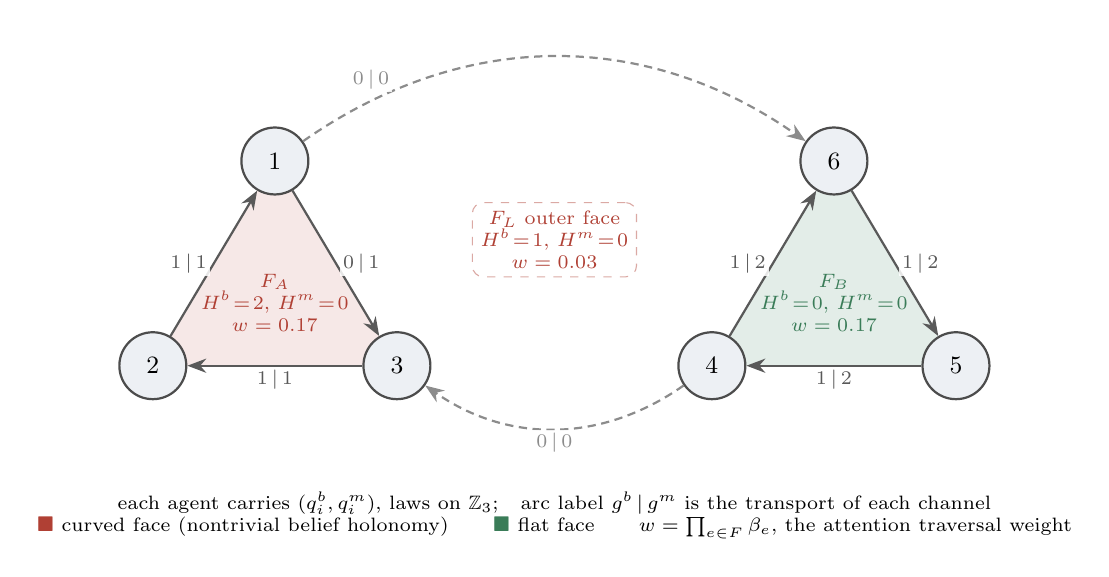
\begin{tikzpicture}[
  >={Stealth[length=2.4mm]},
  every node/.style={font=\small},
  ag/.style={circle, draw=black!70, thick, fill=softg,
             minimum size=8.5mm, inner sep=0pt, font=\small},
  arc/.style={->, thick, black!65},
  cross/.style={->, thick, black!45, densely dashed},
  lab/.style={font=\scriptsize, inner sep=1.2pt, fill=white, fill opacity=0.85,
              text opacity=1},
]
\node[ag] (a1) at (0,1.75)      {$1$};
\node[ag] (a2) at (-1.55,-0.85) {$2$};
\node[ag] (a3) at (1.55,-0.85)  {$3$};
\node[ag] (a4) at (5.55,-0.85)  {$4$};
\node[ag] (a5) at (8.65,-0.85)  {$5$};
\node[ag] (a6) at (7.10,1.75)   {$6$};

\begin{scope}[on background layer]
  \fill[openc!12] (a1.center) -- (a3.center) -- (a2.center) -- cycle;
  \fill[parent!14] (a4.center) -- (a6.center) -- (a5.center) -- cycle;
\end{scope}

\draw[arc] (a1) -- node[lab, pos=.5, right=1pt] {$0\,|\,1$} (a3);
\draw[arc] (a3) -- node[lab, pos=.5, below=0pt] {$1\,|\,1$} (a2);
\draw[arc] (a2) -- node[lab, pos=.5, left=1pt] {$1\,|\,1$} (a1);
\draw[arc] (a4) -- node[lab, pos=.5, left=1pt] {$1\,|\,2$} (a6);
\draw[arc] (a6) -- node[lab, pos=.5, right=1pt] {$1\,|\,2$} (a5);
\draw[arc] (a5) -- node[lab, pos=.5, below=0pt] {$1\,|\,2$} (a4);

\draw[cross] (a1) to[out=35, in=145]
  node[lab, pos=.18, above left=-1pt] {$0\,|\,0$} (a6);
\draw[cross] (a4) to[out=-145, in=-35]
  node[lab, pos=.5, below=0pt] {$0\,|\,0$} (a3);

\node[font=\scriptsize, align=center, openc] at (0,-0.05)
  {$F_A$\\$H^b\!=\!2$, $H^m\!=\!0$\\$w=0.17$};
\node[font=\scriptsize, align=center, parent] at (7.10,-0.05)
  {$F_B$\\$H^b\!=\!0$, $H^m\!=\!0$\\$w=0.17$};
\node[font=\scriptsize, align=center, openc, draw=openc!45, dashed,
      rounded corners, fill=white, inner sep=3pt] at (3.55,0.75)
  {$F_L$ outer face\\$H^b\!=\!1$, $H^m\!=\!0$\\$w=0.03$};

\node[align=center, font=\scriptsize] at (3.55,-2.75) {%
  each agent carries $(q^b_i,q^m_i)$, laws on $\mathbb Z_3$;\quad
  arc label $g^b\,|\,g^m$ is the transport of each channel\\
  \textcolor{openc}{$\blacksquare$}~curved face (nontrivial belief holonomy)\qquad
  \textcolor{parent}{$\blacksquare$}~flat face\qquad
  $w=\prod_{e\in F}\beta_e$, the attention traversal weight};
\end{tikzpicture}
\caption{\textbf{The finite categorical system.} Six agents on two directed
three-cycles joined by two cross arcs, with one $\mathbb Z_3$ element per arc per
channel. The skeleton has three simple directed cycles, equal to its cycle rank, so
its faces form a basis. The belief connection is curved on $F_A$ and on the outer
face $F_L$ and flat on $F_B$; the model connection is flat on every face. Cycle $B$
carries nonzero transports on every arc and still has trivial holonomy, which is
what separates curvature from mere nonidentity. Each face also carries an attention
weight, the probability that the attention walk traverses it, so the long outer face
is suppressed by roughly a factor of six.}
\label{fig:system}
\end{figure}

The faces are where the gauge content lives. A face is a simple directed cycle of the
skeleton; there are three of them here and the cycle rank is also three, so they form
a basis with no redundancy. Each face carries a holonomy from the connection and a
coupling from the attention, and the two are independent: $F_B$ is fully attended and
perfectly flat, while $F_L$ is curved and barely attended. Pairing them gives a
Wilson action, a sum over faces of the traversal weight times the normalized
character defect, which is gauge invariant because both factors are. On this system
the model action is exactly zero and the belief action is positive and dominated by
the short curved face.

What the measurements found separates cleanly. The exact finite layer survives every
check: the tower accounting identity holds to $10^{-15}$, nested coarse-grainings
compose, the dressed-transport law normalizes only when the endpoint factor is
carried, and the predicted belief-against-model asymmetry is directly observable.
The block-formation story does not survive in the form the design anticipated.
Eliminating the block parent exactly generates a three-body term, so pairwise closure
is false here. There is no timescale separation between partition persistence and
belief relaxation. And the designed partition into the two cycles is never selected,
for a reason that is structural rather than incidental: that partition contains the
curved block, so every curvature charge taxes it, and a mechanism that penalizes
enclosed curvature necessarily pushes away from the blocks the design named. An
observable asymmetry is not a selected one.

The most useful thing to come out of the sweep is that the declared knobs are not
independent. At the transition between keeping the curved loop inside one block and
cutting it, the curvature charge carried by that block plus the log of the partition
prior's concentration is a single constant, and this holds whether the charge is
bought with a retention price against the holonomy group or with a Wilson coupling
against the attention-weighted faces. Only the sum matters. That sharpens
Corollary~6 rather than escaping it: selection still lives entirely in declared
structure, but the structure is now one number with three interchangeable dials, one
of which is the attention. The dynamics does not yet carry the Wilson term, so the
persistence and null-control results above describe the earlier energy and should not
be reread in its light.

\subsection{Why the coarse theory is not pairwise}

The statement that exact closure generates many-body terms is easy to misread off
the architecture, so it is worth locating precisely. Looking at the two blocks of
the declared instance one sees two meta-agents joined by two cross arcs, which is a
pairwise coupling, and that reading is correct. The generated three-body term is
not there. It sits \emph{inside} a block, among the three children of one parent,
and deleting both cross arcs leaves it bit-identical.

\begin{figure}[t]
\centering
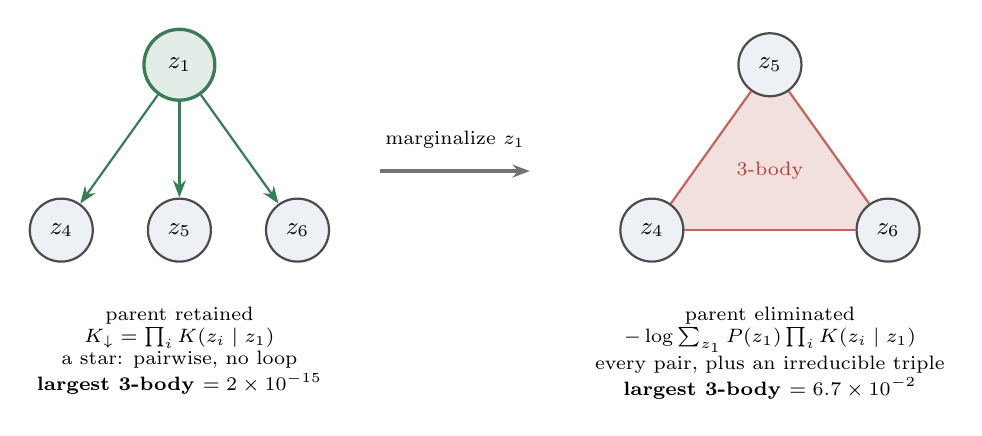
\begin{tikzpicture}[
  >={Stealth[length=2.2mm]},
  every node/.style={font=\small},
  ch/.style={circle, draw=black!70, thick, fill=softg,
             minimum size=8mm, inner sep=0pt, font=\small},
  pa/.style={circle, draw=parent, very thick, fill=parent!14,
             minimum size=9mm, inner sep=0pt, font=\small},
  down/.style={->, thick, parent},
  pair/.style={-, thick, openc!80},
]
\node[pa] (p) at (0,1.9) {$z_1$};
\node[ch] (c4) at (-1.5,-0.2) {$z_4$};
\node[ch] (c5) at (0,-0.2)    {$z_5$};
\node[ch] (c6) at (1.5,-0.2)  {$z_6$};
\draw[down] (p) -- (c4);
\draw[down] (p) -- (c5);
\draw[down] (p) -- (c6);
\node[font=\scriptsize, align=center, anchor=north] at (0,-1.05) {%
  parent retained\\
  $K_\downarrow=\prod_i K(z_i\mid z_1)$\\
  a star: pairwise, no loop\\[1.5pt]
  \textbf{largest 3-body $=2\times10^{-15}$}};

\node[font=\scriptsize, align=center] at (3.5,0.95) {marginalize $z_1$};
\draw[->, very thick, black!55] (2.55,0.55) -- (4.45,0.55);

\node[ch] (d4) at (6.0,-0.2)  {$z_4$};
\node[ch] (d6) at (9.0,-0.2)  {$z_6$};
\node[ch] (d5) at (7.5,1.9)   {$z_5$};
\begin{scope}[on background layer]
  \fill[openc!16] (d4.center) -- (d5.center) -- (d6.center) -- cycle;
\end{scope}
\draw[pair] (d4) -- (d5);
\draw[pair] (d5) -- (d6);
\draw[pair] (d4) -- (d6);
\node[font=\scriptsize, openc] at (7.5,0.55) {3-body};
\node[font=\scriptsize, align=center, anchor=north] at (7.5,-1.05) {%
  parent eliminated\\
  $-\log\sum_{z_1}P(z_1)\prod_i K(z_i\mid z_1)$\\
  every pair, plus an irreducible triple\\[1.5pt]
  \textbf{largest 3-body $=6.7\times10^{-2}$}};
\end{tikzpicture}
\caption{\textbf{A hub, eliminated.} The downward kernel factorizes over children
given the parent, so with the parent retained the block is a star and the children
are conditionally independent: the measured three-body coefficient is at the
arithmetic noise floor. Marginalizing the parent couples everything it touched, all
at once rather than pairwise, and an irreducible triple appears fourteen orders of
magnitude above that floor. The higher-order structure is the price of describing
the children without naming the parent.}
\label{fig:star}
\end{figure}

The mechanism is the one shown in Figure~\ref{fig:star}. The downward kernel
factorizes over children given the parent, so conditionally on $z_1$ the children
are independent and the block is a star, which is pairwise and carries no loop.
Marginalizing the parent leaves $-\log\sum_{z_1}P(z_1)\prod_i K(z_i\mid z_1)$,
which is not additively separable in the children. A common cause, once integrated
out, couples everything it touched simultaneously.

This is the Ising star exactly: one center spin coupled to three leaves, eliminate
the center, and a genuine three-leaf term
$2\,\mathrm{sech}^2(h_0)\tanh(h_0)J_1J_2J_3$ appears at leading order. The exact
coefficient of the finite model converges to that closed form as the couplings
shrink, with successive ratios $0.470$, $0.815$, $0.951$, $0.988$, $0.997$ over
halvings of the coupling scale, and vanishes exactly when the field or any one
coupling does.

Both statements are therefore true at once, at different levels. At the coarse
level the two meta-agents are joined pairwise. At the fine level the exact
effective theory on the children, after parents are eliminated, is not pairwise.
It is the second that obstructs iteration: a pairwise scale-zero theory produces a
scale-one theory outside the pairwise family, so the same machinery cannot simply
be applied again. This is an obstruction to a second scale independent of the
missing rescaling map.

Two measurements qualify how severe it is, and they disagree in an informative
way. Unweighted, the interaction coefficients do not decay with order at all: on a
five-agent block the one- through five-body magnitudes are $0.93$, $1.61$, $0.85$,
$1.62$ and $0.64$, so there is no small parameter organizing a hierarchy of the
kind an effective field theory relies on. Weighted by the Boltzmann measure the
model itself assigns, the omitted three-and-higher content is about two percent of
the retained flow. The higher-order terms are large in magnitude and concentrated
where the measure is small. Whether truncation is controlled therefore depends on
the norm, and in the norm that governs expectations it appears to be.

None of this licenses calling the construction nonrenormalizable. That is a
statement about a flow: linearize about a fixed point, count relevant directions,
find infinitely many. With no rescaling map and no fixed point, the question
cannot be posed. Generated operators are in any case universal rather than
diagnostic, since real-space decimation of an Ising model generates four-spin
couplings and that model is perfectly renormalizable; what separates the cases is
whether the generated operators are irrelevant, which is exactly what cannot be
asked here. The tower also terminates at $N$-body on $N$ agents rather than
continuing indefinitely, and a finite system at one contextual point has no short
distance for a nonrenormalizability statement to be about.

\section{Confidence and provenance}

The exact finite derivations are explicit and internally checked, and several related
finite results are certified in other released derivation packages. The most recent
package covering the multiscale construction released with terminal status
\textsc{inconclusive}, and no claim in it carries a verified state, because no
independent model checked the derivations. An external review of that package found
four substantive defects and six lesser ones, all now repaired; one of the four had
been raised by the package's own adversarial pass and then wrongly dismissed on a
repair that was described but never implemented. That episode is the reason for the
reporting discipline in this note: treat the finite layer as the current author-derived
working calculus, not as an independently certified package, and treat claims of
persistence, emergent hierarchy, or physical RG flow as unproved until a specific
obligation in the table above is discharged.

\end{document}
